\documentclass{article}

\usepackage[a4paper]{geometry}
\usepackage[ngerman]{babel}
\usepackage[utf8]{inputenc}
\usepackage[T1]{fontenc}
\usepackage{graphicx}
\usepackage{fancyhdr}
\usepackage{xcolor}
\usepackage{float}

\graphicspath{{./images/}}

\pagestyle{fancyplain}
\fancyhf{}
\lhead{\fancyplain{}{Mara Schulke} }
\rhead{\fancyplain{}{\today}}
\cfoot{\fancyplain{}{\thepage}}

\begin{document}

\begin{titlepage}
	\begin{flushleft}
		TH Brandenburg \\
		Studiengang IT Sicherheit \\
		Fachbereich Informatik und Medien \\
		Entwicklung Sicherer Softwaresysteme \\
		Prof. Dr.-Ing. Martin Schafföner
	\end{flushleft}

	\vfill

	\begin{center}
		\Large{Einsendeaufgabe: Threat Analysis}\\[0.5em]
		\large{Sommersemester 2024}\\[0.25em]
		\large{Abgabetermin \today}
	\end{center}

	\vfill

	\begin{flushright}
		Mara Schulke \\
		Matrikel-Nr. 20215853
	\end{flushright}
\end{titlepage}

\begin{abstract}
	In dieser Einsendeaufgabe wird die Online-Meeting-Plattform Google Meet der Firma 
	Google hinsichtlich ihrer softwareseitigen Risiken und Gefahren analysiert.
	Es wird die Vorgehensweise der Gefahrenanalyse, die entdeckten Risiken und Gefahren 
	zusammengefasst und eine Priorisierung mit Handlungsempfehlung daraus abgeleitet. Des 
	weiteren wird auf die Methodik der Gefahrenanalyse eingegangen und von alternativen 
	Vorgehensweisen abgegrenzt.
\end{abstract}

\tableofcontents

\listoffigures

\section{Projektauswahl: Google Meet}

Die Auswahl des zu analysierenden Projektes fiel auf die Online-Meeting-Plattform Google 
Meet, da diese mehrere Punkte abdeckt:

\begin{enumerate}
	\item Ihre Funktionsweise- und -umfang ist ihm Rahmen einer Kurzanalyse greifbar
	\item Die Anwendungsarchitektur lässt sich aus vergleichbaren Echtzeit-Meeting Anwendungen ableiten und vereinfachen
	\item Sie hat einen weitreichenden Bekanntheitsgrad
\end{enumerate}

Vereinfacht lässt sich Google Meet in einer Client-Server Architektur darstellen, auch 
wenn an dieser Stelle angemerkt werden muss, dass durch die Menge an Nutzern, die Vielzahl 
an Integrationen und die Stabilität der Software davon auszugehen ist, dass es sich nicht 
um eine naive Architektur der Server bzw. Server-Infrastruktur handelt. 

Im Rahmen dieser Einsendeaufgabe wird die Annahme getroffen, dass Google Meet der 
folgenden Architektur entlang aufgebaut ist:

\begin{figure}[H]
	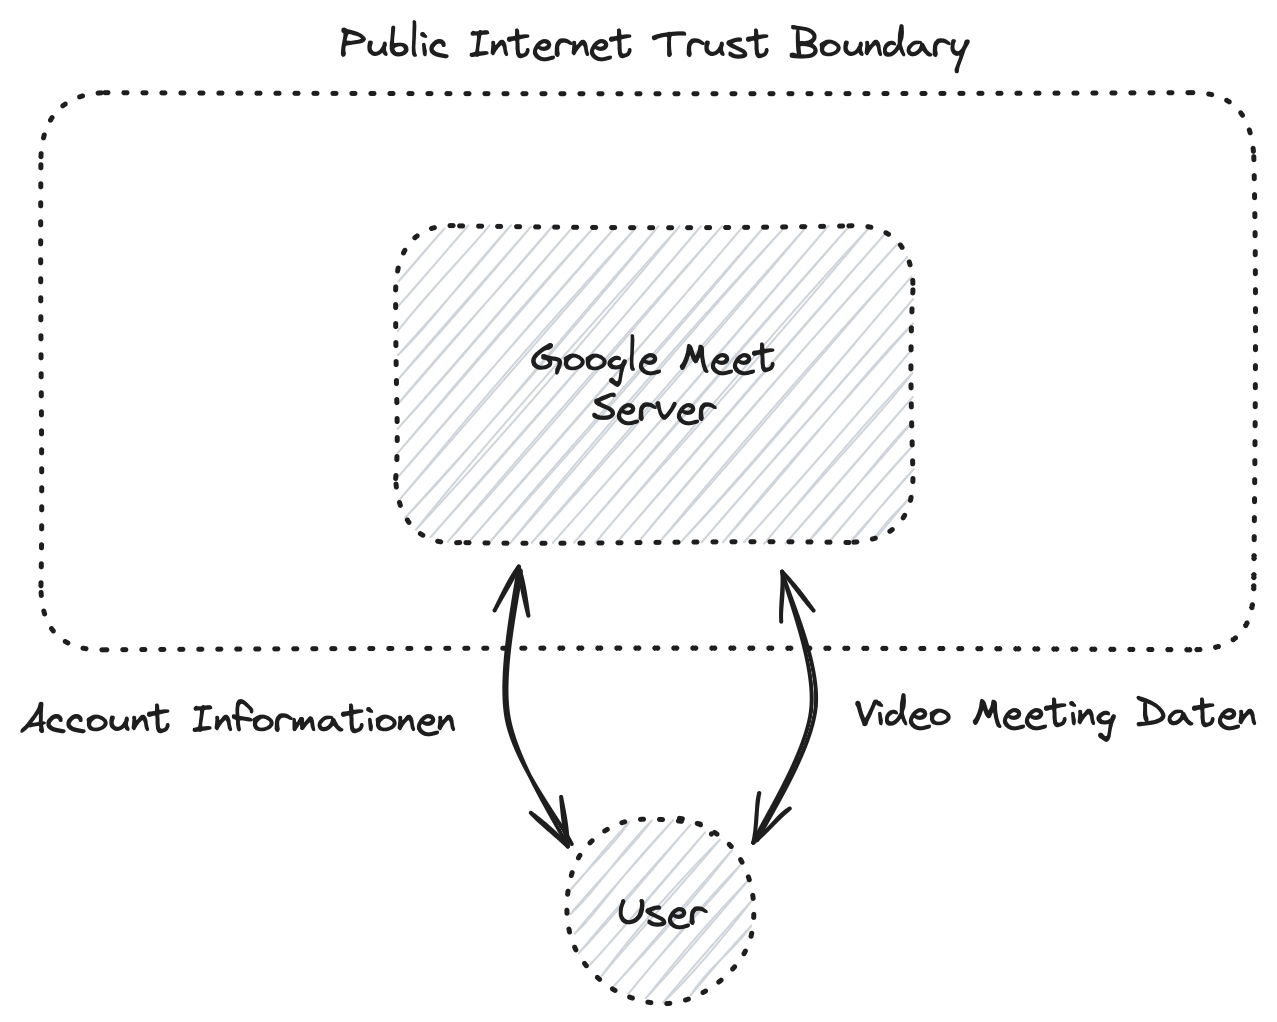
\includegraphics[width=0.75\textwidth]{./google-meet-diagram.png}
	\centering
	\caption{Anwendungsarchitektur Google Meet (stark vereinfacht)}
\end{figure}

Im Rahmen dieser Aufgabe wird von einer monolithischen Anwendungsarchitektur von Google 
Meet ausgegangen in einem zeitlich angemessenen Rahmen in der Lage zu sein eine 
hypothetische Gefahrenanalyse durchführen zu können. Der Google Meet Server in der 
beistehenden Grafik übernimmt die Verwaltung der Sitzungen, die Account-Authentifizierung 
und die Aushandlung der WebRTC-Sitzungen zwischen verschiedenen Nutzer.

\section{Auswahl der Gefahrenanalyse Software}

Um eine automatisierte Gefahrenanalyse durchzuführen stehen mittlerweile (Stand Mai 2024), 
eine Vielzahl an verschiedenen Tools zur Verfügung. Nachfolgend sind einige beliebte 
bzw. bekannte, kostenlose \textit{Threat-Modelling}-Programme aufgelistet:

\subsection*{Kostenlose Software}

Da diese Einsendeaufgabe von geringem Umfang ist und keine weiteren Anwendungsfälle für 
eine ausgereifte Threat-Modelling Software absehbar sind beschränke ich den Vergleich 
verschiedener Software-Lösungen auf kostenlose bzw. Open-Source Programme.

\subsubsection*{MTMT – Microsoft Threat Modeling Tool}

MTMT ist das Threat Modeling Tool der Firma Microsoft. Es ist ein weit verbreitetes 
Werkzeug zur Modellierung von Software und der Automatisierten Analyse dieser Modelle. Da 
der Anbieter Microsoft ist, besteht leider die Anforderung MTMT auf einem Windows-System 
auszuführen.

Das MTMT ist weiterhin ein sehr umfangreiches Werkzeug, das ebenfalls im professionellen 
Kontext Einsatz findet – dies resultiert in einer komplexen Oberfläche mit 
vielen Möglichkeiten und ausgereiften Konzepten.

Leider musste ich durch die Gegebenheit, kein Windows-System zu betreiben, die Analyse 
des MTMT hier beenden, da es mir leider nicht möglich war eine ausführbare Version für 
Unix-Systeme zu finden ohne Virtualisierung zu verwenden.

\subsubsection*{OWASP ThreatDragon}

OWASP ThreatDragon ist eine Software der Organization OWASP (kurz für \textit{Open 
Worldwide Application Security Project}). Die Software ist kostenlos und
Browser basiert. Sie enthält Funktionen für die Diagramm-Zeichnung und anschließende 
Erstellung eines Sicherheits-Reports. Die Arbeitsstände müssen allerdings immer 
heruntergeladen werden und in lokalen Dateien gespeichert werden – dies ist eine relativ 
umständliche Arbeitsweise, da anders als bei nativer Software nicht eine Datei durchgehend 
geöffnet und bearbeitet werden kann. Außerdem bietet ThreatDragon nur einen begrenzten 
Umfang an erkannten Sicherheitslücken bei einer offensichtlich fehlerhaften 
Softwarearchitektur.

\subsubsection*{AWS ThreatComposer}

AWS ThreatComposer ist eine Open Source Software der Firma Amazon. Sie ist ebenfalls 
Browser basiert, allerdings etwas ausgereifter und nutzerfreundlicher als die OWASP 
alternative. Dennoch gibt es auch hier einige Unannehmlichkeiten für Nutzer: Die 
Benutzeroberfläche ist unklar (e.g. Diagramme sind nur zur Dokumentation hinzuzufügen, 
nicht zur automatisierten Auswertung). Es gibt keine klare Datenverwaltung bzw. keinen 
klaren Datenexport und der allgemeine Funktionsumfang wirkt etwas eingeengt.

\subsubsection*{Threagile}

Threagile ist kostenlose Open-Source Software zur Gefahrenanalyse ohne eine 
Benutzeroberfläche. Dies ist eine Eigenheit im Vergleich zu den anderen vorgestellten 
Programmen die hauptsächlich über das Desktop- oder Web-Interface zu bedienen sind.
Threagile lässt sich über eine .yaml Datei bedienen die einem vorgegebenen Schema 
entsprechen muss. So lassen sich im Quelltext Komponenten (und ihre Beziehungen), 
Datenbanken, Verschlüsselungen, Datenflüsse, verwendete Technologien und vieles mehr 
Dokumentieren.

Der klare Vorteil von Threagile liegt in der Möglichkeit diese YAML-Datei bzw. die 
analysierte Architektur ohne weiteres in git oder anderen VCS (kurz für \textit{Version 
Control Systems}) zu versionieren. Bei anderer proprietär Software ist dies zwar 
grundsätzlich Möglich aber da VCS in der Regel auf Klartext-Dateien ausgelegt sind sind 
die Möglichkeiten begrenzt bzw. parallel im Team an einer Datei zu arbeiten.

Des Weiteren ist es einfach mittels Threagile eine Gefahrenanalyse auf der YAML-Datei 
auszuführen und der generierte Report hat eine hohe Qualität (optisch, strukturell und 
inhaltlich).

\subsection{Begründung der Auswahl}

Im Rahmen dieser Einsendeaufgabe habe ich mich unter den oben dargestellten Abgrenzungen 
der verschiedenen Softwarelösungen für die Nutzung von Threagile entschieden. Threagile 
ist einfach zu bedienen, reproduzierbar (mittels Docker), eine nützliche Resource für 
zukünftige berufliche Situationen.

\section{Ergebnis der automatisierten Gefahrenanalyse}

Der automatisierte Report von Threagile hat basierend der oben dargestellten, stark 
vereinfachten, Anwendungsarchitektur hat insgesamt 21 mögliche Risiken und in 12 
verschiedenen Risiko-Klassen identifizieren können.

Folgende Risiko-Klassen wurden mit der Stufe \textit{Elevated – Wahrscheinlicher Angriff mit hohem Schaden} markiert:

\begin{enumerate}
	\item Cross-Site-Scripting 
	\item Missing Cloud Hardening
	\item Missing Hardening
	\item Server-Side-Request-Forgery
\end{enumerate}

Alle anderen entdeckten Risiko-Klassen wurden mit der Stufe \textit{Medium – Unwahrscheinlicher Angriff mit hohem Schaden} markiert:

\begin{enumerate}
	\item Container Base Image Backdooring
	\item Cross-Site-Request-Forgery
	\item DoS-Risky Access Across Trust Boundary
	\item Missing Identity Propagation
	\item Missing Identity Provider Isolation
	\item Missing Two-Factor Authentication
	\item Missing Vault
	\item Mixed Targets on Shared-Runtime
\end{enumerate}

Zusammenfassend lässt sich über die entdeckten Risiken sagen, dass diese ein konkretes,
greifbares Risiko darstellen und Threagile wenige ``False-Positives'' entdeckt hat (bspw. 
Fehler die lediglich aufgrund einer Ungenauigkeit der Diagramm-Funktion markiert werden). 
Threagile lässt eine sehr detaillierte Dokumentation von Verschlüsselungs-Methoden, 
übertragenen Datensätzen und verwendeten Datenformaten etc. zu. Die Liste der einzelnen 
Risiken finden sie im Threagile-Report (Anhang 1). 

\section{Priorisierung der Gefahren}

Die logische Schlussfolgerung der oben eingestuften Risiko-Klassen ist die priorisierung 
der Gefahren nach absolutem Risiko:

$$Risiko = Schaden * Wahrscheinlichkeit$$

\vspace{0.5em}

Demzufolge bezieht sich diese Priorisierung lediglich auf die Gefahren aus der Klasse 
\textit{Elevated}:

\begin{enumerate}
	\item Cross-Site Scripting (XSS) risk at Google Meet Server (\textit{Likely with High impact})
	\item Missing Cloud Hardening risk at Google Cloud (\textit{Unlikely with Very High impact})
	\item Missing Cloud Hardening risk at Public Internet (\textit{Unlikely with Very High impact})
	\item Cross-Site Scripting (XSS) risk at Auth Server (\textit{Likely with Medium impact})
	\item Missing Hardening risk at Google Meet Server (\textit{Likely with Medium impact})
	\item Server-Side Request Forgery (SSRF) risk at Auth Server server-side web-requesting the target Google Meet Server via Google Meet Server (\textit{Likely with Medium impact})
	\item Server-Side Request Forgery (SSRF) risk at Google Meet Server server-side web-requesting the target Auth Server via User Authentication Access: (\textit{Likely with Medium impact})
	\item Server-Side Request Forgery (SSRF) risk at Google Meet Server server-side web-requesting the target Google Meet Client via Web Interface (\textit{Likely with Medium impact})
\end{enumerate}

\section{Detaillierte Betrachtung}

\subsection{Cross-Site-Scripting (XSS)}

Da Google Meet text-basierte Nutzereingaben als eine der Kernfunktionen (Chat) zulässt, 
stellt Cross-Site-Scripting ein erhebliches Risiko dar. Allerdings muss an dieser Stelle
angemerkt werden, dass die Empfänger einer bösartigen lediglich die Nutzer einer Sitzung 
sind (meist, ein bis zweistellige Nutzerzahlen) – wohingegen auf Plattformen wie Twitter 
und YouTube etc. Nutzer öffentlich Beiträge posten können was die Anzahl an betroffenen 
Nutzern drastisch erhöht.

Davon unberührt ist allerdings die Ausführung von Code bzw. Befehlen auf dem Google 
Meet Server (auch bekannt als \textit{RCE – Remote Code Execution}) mittels XSS.

\subsection{Missing Cloud Hardening}

Die fehlende Absicherung der Cloud gegen unbefugten Zugriff (bspw. via SSH, 
Netzwerkschwachstellen etc) stellt neben XSS die größte Gefahr dar, da diese mit einer 
möglichen ``Escalation of Privilege'' einhergehen könnte und somit ein Angreifer nach der 
infiltration einer der Cloud-Internen-Komponenten wohlmöglich weitere Komponenten 
infizieren könnte. Mögliche Lösungsstrategien zur Absicherung der Cloud bestehen darin,
verwaltete Services (für Netzwerkverbindungen, Datenbanken, Load-Balancing, Server-
Hosting) der GCP in Anspruch zu nehmen, anstatt mittels VM eine manuelle Infrastruktur 
einzurichten. Bei Verwendung der verwalteten Lösungen (was bei Google's eigener Software 
sehr wahrscheinlich ist) besteht keine Notwendigkeit, dass sich das Google Meet Team um 
Updates der Netzwerk-Software, Firewall etc. kümmert. 

Threagile schlägt zur Unterbindung dieser Gefahr vor, bekannte Absicherungs-Frameworks 
(unteranderem von OWASP) zu verwenden, um die cloud-interne Architektur zu überprüfen.

\section{Zusammenfassung}

Insgesamt lassen sich aus dem generierten Threagile-Report mit wenig Aufwand wichtige 
Hinweise zu grundlegenden Problemen der verwendeten Software-Architektur ableiten. Da 
Threagile gleichzeitig zur internen Dokumentation und zur Gefahrenanalyse verwendet werden 
kann, bietet die Nutzung eine 

\end{document}
